\documentclass[12pt]{article}
\usepackage{graphicx}
\usepackage{amsmath}
\usepackage[framed]{matlab-prettifier}

\begin{document}
\begin{titlepage}
	\begin{center}
	\line(1,0){300}\\
	[0.25in]
	\huge{\bfseries Lab 1: Kinematic Characterization of the Lynx (MATLAB)}\\
	[0.12in]
	\line(1,0){200}\\
	[1cm]
	\textsc{\Large University of Pennsylvania}\\
	\end{center}
	\vfill
	\begin{flushright}
	\textsc{\large Wesley Yee, Shaun Fedrick\\
	MEAM 520\\
	September 23, 2020\\}
	\end{flushright}
\end{titlepage}

\section{Methods}
For our experimental setup, we used MATLAB to code our forward kinematics calculations, which communicated to ROS running via Gazebo on a local VM running Ubuntu. A 6-DOF robot arm manipulator was programmed to run in Gazebo. Once the code was run in MATLAB on the host computer, the commands for operating the robot were then sent to Gazebo which then actuated the robot to the desired joint variable positions. \\ \\
The ROS robot was modeled off of an actual physical robot located at Penn, but was not accessible due to COVID-19.
\begin{enumerate}
\item \begin{figure} [h]
	\centering 
	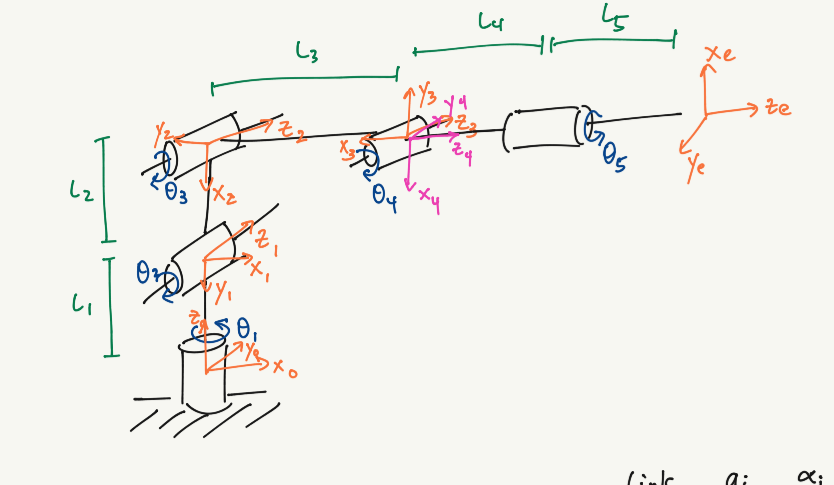
\includegraphics[scale=1]{Q1.png}
	\caption{Revised symbolic representation}
	\end{figure}
\item FIX THESE BELOW
\begin{equation}
	T^{0}_{1} = \begin{bmatrix}
	0 & 0 & 1 & 0mm\\
	-1 & 0 & 0 & 0mm\\
	0 & -1 & 0 & 76.2mm\\
	0 & 0 & 0 & 1
	\end{bmatrix}
\end{equation}
\begin{equation}	
	T^{1}_{2} = \begin{bmatrix}
	0 & -1 & 1 & 0mm\\
	1 & 0 & 0 & 146.05mm\\
	0 & 0 & 1 & 0mm\\
	0 & 0 & 0 & 1
	\end{bmatrix}
\end{equation}
\begin{equation}	
	T^{2}_{3} = \begin{bmatrix}
	-\frac{\sqrt{2}}{2} & -\frac{\sqrt{2}}{2} & 0 & -132.4588mm\\
	\frac{\sqrt{2}}{2} & -\frac{\sqrt{2}}{2} & 0 & 132.4588mm\\
	0 & 0 & 1 & 0mm\\
	0 & 0 & 0 & 1
	\end{bmatrix}
\end{equation}

\begin{equation}	
	T^{3}_{4} = \begin{bmatrix}
	0 & 0 & -1 & 0mm\\
	-1 & 0 & 0 & 132.4588mm\\
	0 & 1 & 0 & 0mm\\
	0 & 0 & 0 & 1
	\end{bmatrix}
\end{equation}

\begin{equation}	
	T^{4}_{5} = \begin{bmatrix}
	0 & 1 & 0 & 0mm\\
	-1 & 0 & 0 & 0mm\\
	0 & 0 & 1 & 68mm\\
	0 & 0 & 0 & 1
	\end{bmatrix}
\end{equation}

\begin{equation}	
	T^{4}_{5} = \begin{bmatrix}
	-1 & 0 & 0 & 0mm\\
	0 & \frac{\sqrt{2}}{2} & -\frac{\sqrt{2}}{2} & 84.3755mm\\
	0 & -\frac{\sqrt{2}}{2} & -\frac{\sqrt{2}}{2} & 14.5255mm\\
	0 & 0 & 0 & 1
	\end{bmatrix}
\end{equation}
\item 
\item 
\end{enumerate}

\section{Results}


\section{Evaluation}
\begin{enumerate}
\item
\begin{equation}	
	T^{0}_{e} = \begin{bmatrix}
	0 & 0 & 1 & 255.325mm\\
	0 & -1 & 0 & 0mm\\
	1 & 0 & 0 & 222.25mm\\
	0 & 0 & 0 & 1
	\end{bmatrix}
\end{equation}
\item
\begin{enumerate}
\item
\begin{equation}	
	T^{0}_{e} = \begin{bmatrix}
	0 & \frac{\sqrt{2}}{2} & \frac{\sqrt{2}}{2} & 180.542mm\\
	0 & -\frac{\sqrt{2}}{2} & \frac{\sqrt{2}}{2} & 180.542mm\\
	1 & 0 & 0 & 222.25mm\\
	0 & 0 & 0 & 1
	\end{bmatrix}
\end{equation}
\item
\begin{equation}	
	T^{0}_{e} = \begin{bmatrix}
	-1 & 0 & 0 & 0mm\\
	0 & \frac{\sqrt{2}}{2} & -\frac{\sqrt{2}}{2} & -180.542mm\\
	0 & -\frac{\sqrt{2}}{2} & -\frac{\sqrt{2}}{2} & 41.708mm\\
	0 & 0 & 0 & 1
	\end{bmatrix}
\end{equation}
\end{enumerate}
\item
\item \begin{figure} [h]
	\centering 
	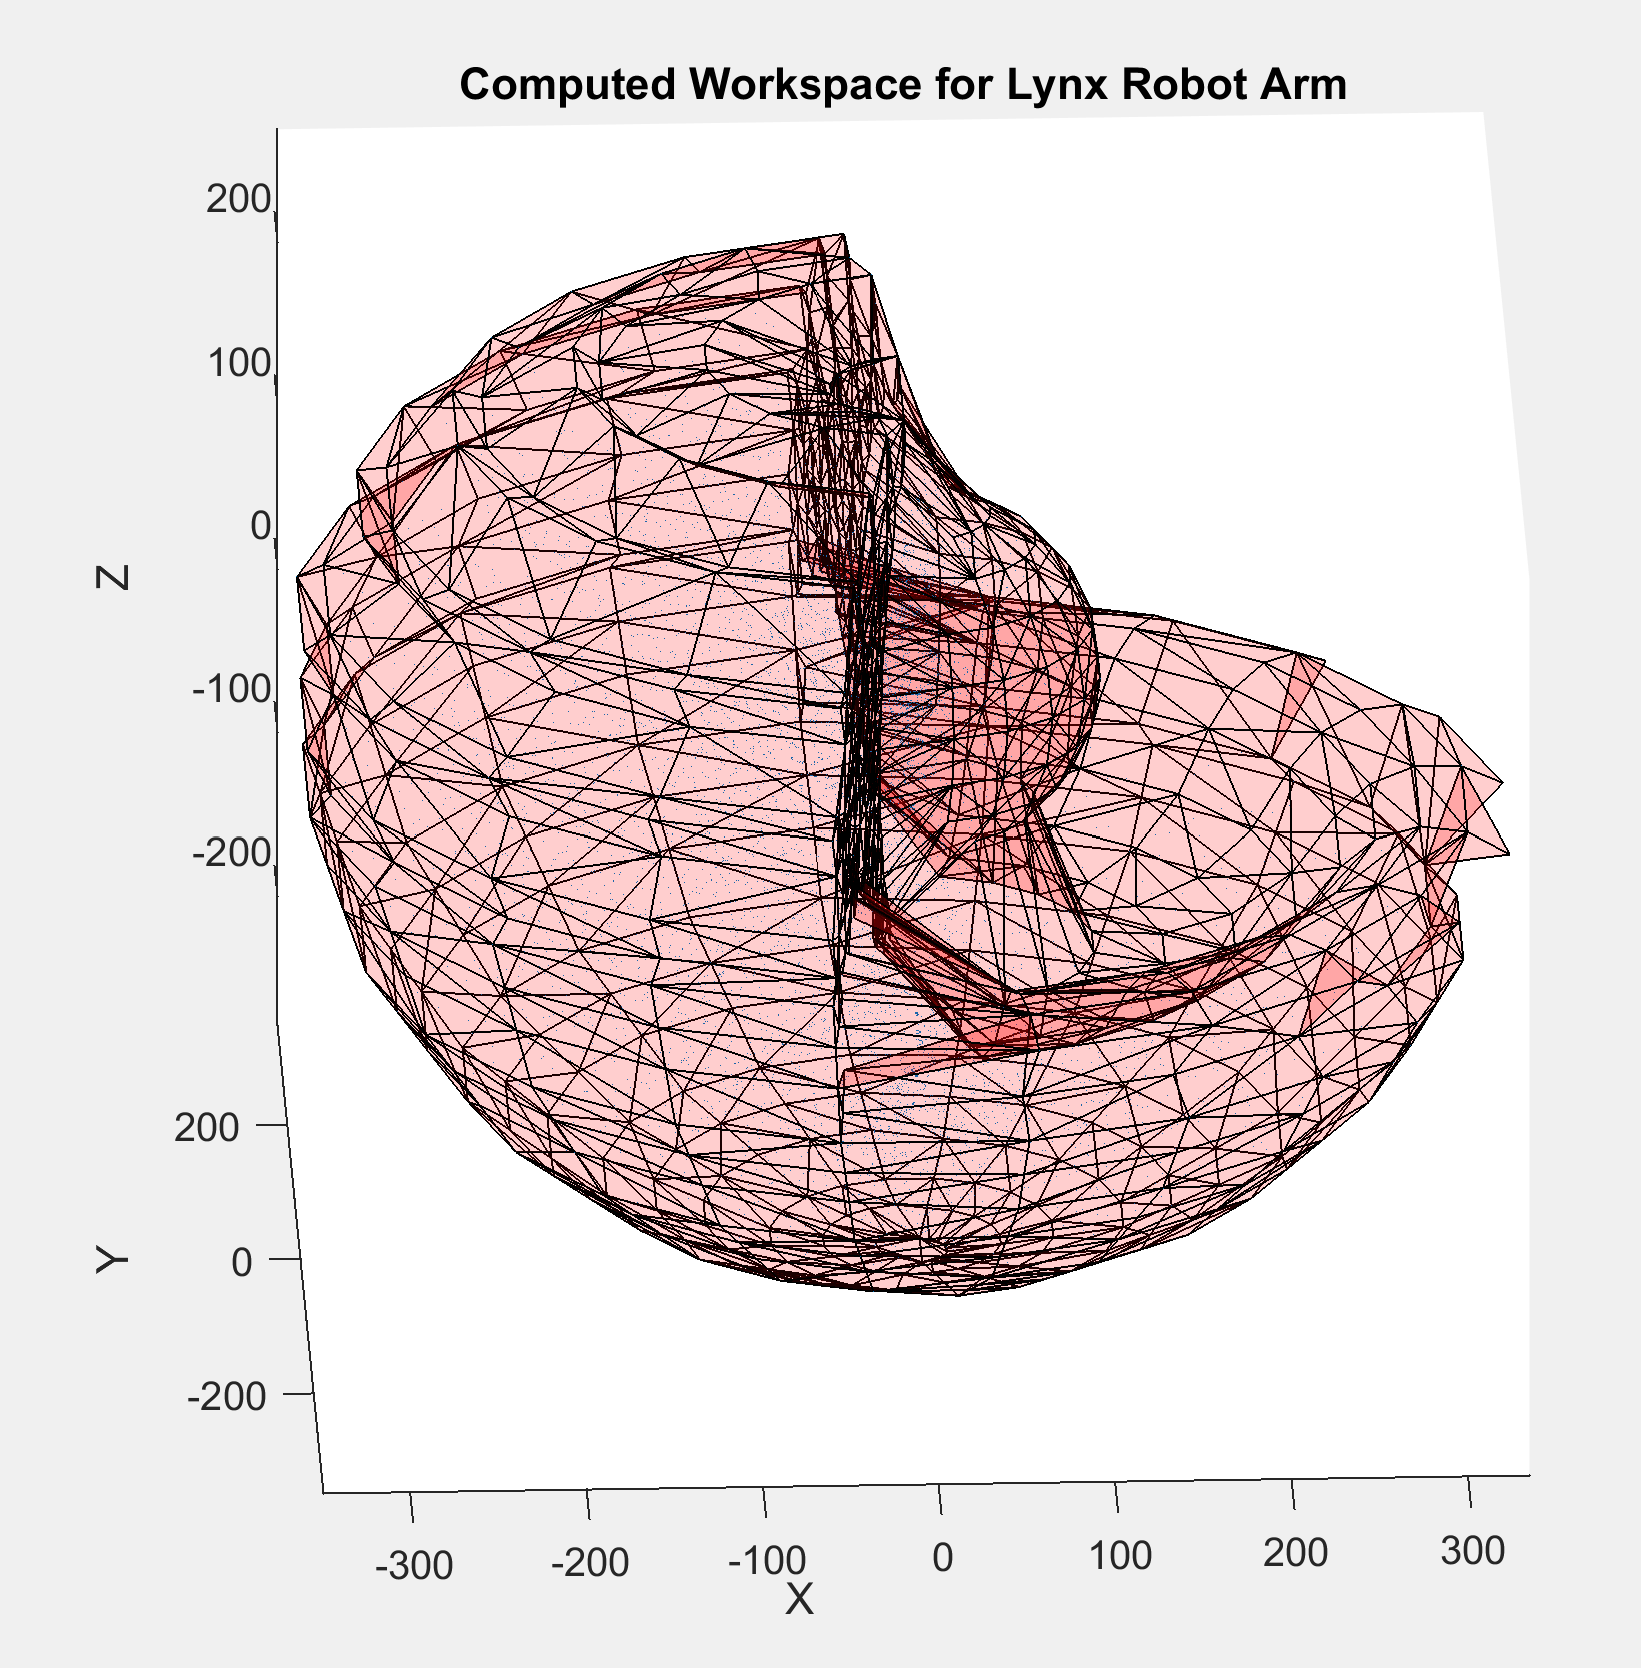
\includegraphics[scale=.5]{ComputedWorkspace.png}
	\caption{Computed Workspace of Lynx Robot}
	\end{figure}
\item As seen in the code below, the predicted joint positions are almost exactly aligned with the simulated joint positions, aside from a 0.002mm difference in the x position of Joint 3. This is negligible and can be explained due to possible compounded rounding errors in the ROS robot.\\ \\ However, when examining the $T^{0}_{e}$ matrices, the Simulation $T^{0}_{e}$ records different values of $x_{0}$ and $y_{0}$ in the end effector frame. We believe that this is due to a mistake in the provided ROS robot code used to calculate Simulation $T^{0}_{e}$. Justification for this conjecture is provided in Problem 1 of the Analysis section.\\

\lstinputlisting[style=Matlab-editor,caption={Outputs of TestFK\_Sim.m for 
	$q = \begin{bmatrix}
	0 & 0 & 0 & 0 & 0 & 0\\
	\end{bmatrix}$}]{24Prob5output.m}


\end{enumerate}

\newpage
\section{Analysis}
\begin{enumerate}
\item As expected, the results of our evaluation were correct. From the figure below, we use Right-Hand Rule convention to establish that the base frame's red axis is $x_{0}$, the green axis is $y_{0}$ and the blue axis is $z_{0}$. The same axes are applied to the end effector frame, respectively. \\\begin{figure} [h]
	\centering 
	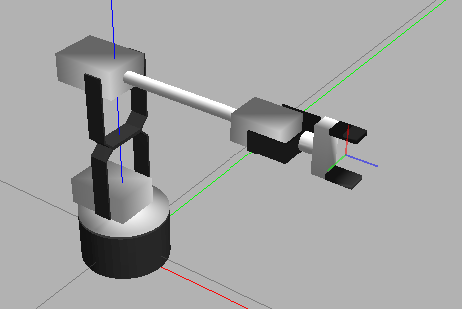
\includegraphics[scale=2]{ImageOfRobotZeroConfig.png}
	\caption{ROS Robot in Zero Configuration}
	\end{figure} \\
If we use these axes to construct a rotation matrix $R$ by observing each end effector's axis' projection on the base frame's axes, we can compute the following rotation matrix:
\\
\begin{equation}
R = \begin{bmatrix}
	0 & 0 & 1 \\
	0 & -1 & 0\\
	1 & 0 & 0
	\end{bmatrix}
\end{equation}
\\
For example, $R$ states that the projection of the end effector's y axis $y_{e}$ is in the opposite direction of the base frame's y axis $y_{0}$. This value validates the Predicted $T^{0}_{e}$ in Analysis Problem 2.4 and shows that the Simulated $T^{0}_{e}$ is incorrect.\\\\Fortunately, as seen in the same problem, the joint positions were not affected by this error.


\item 
\end{enumerate}

\section{Appendix}
\lstinputlisting[style=Matlab-editor,caption={calculateFK.m]{Code/calculateFK.m}
	
\lstinputlisting[style=Matlab-editor,caption={computeWorkspace.m]{Code/computeWorkspace.m}
	
\lstinputlisting[style=Matlab-editor,caption={createA.m]{Code/createA.m}

\end{document}
